% Created 2022-09-20 Tue 12:01
\documentclass[9pt, b5paper]{article}
\usepackage{xeCJK}
\usepackage{minted}
\usepackage[T1]{fontenc}
\usepackage[scaled]{beraserif}
\usepackage[scaled]{berasans}
\usepackage[scaled]{beramono}
\usepackage{graphicx}
\usepackage{xcolor}
\usepackage{multirow}
\usepackage{multicol}
\usepackage{float}
\usepackage{textcomp}
\usepackage{algorithm}
\usepackage{algorithmic}
\usepackage{latexsym}
\usepackage{natbib}
\usepackage{geometry}
\geometry{left=1.2cm,right=1.2cm,top=1.5cm,bottom=1.2cm}
\newminted{common-lisp}{fontsize=\footnotesize} 
\usepackage[xetex,colorlinks=true,CJKbookmarks=true,linkcolor=blue,urlcolor=blue,menucolor=blue]{hyperref}
\author{Heyan Jenny Huang}
\date{\today}
\title{Appellant's Desigtnation of Record on Appeal on Case No. 22-2-00195-38}
\hypersetup{
  pdfkeywords={},
  pdfsubject={},
  pdfcreator={Emacs 27.1 (Org mode 8.2.7c)}}
\begin{document}

\maketitle
\tableofcontents


\section{My Appeal of Stalking protection order Brief Statement and Summary}
\label{sec-1}

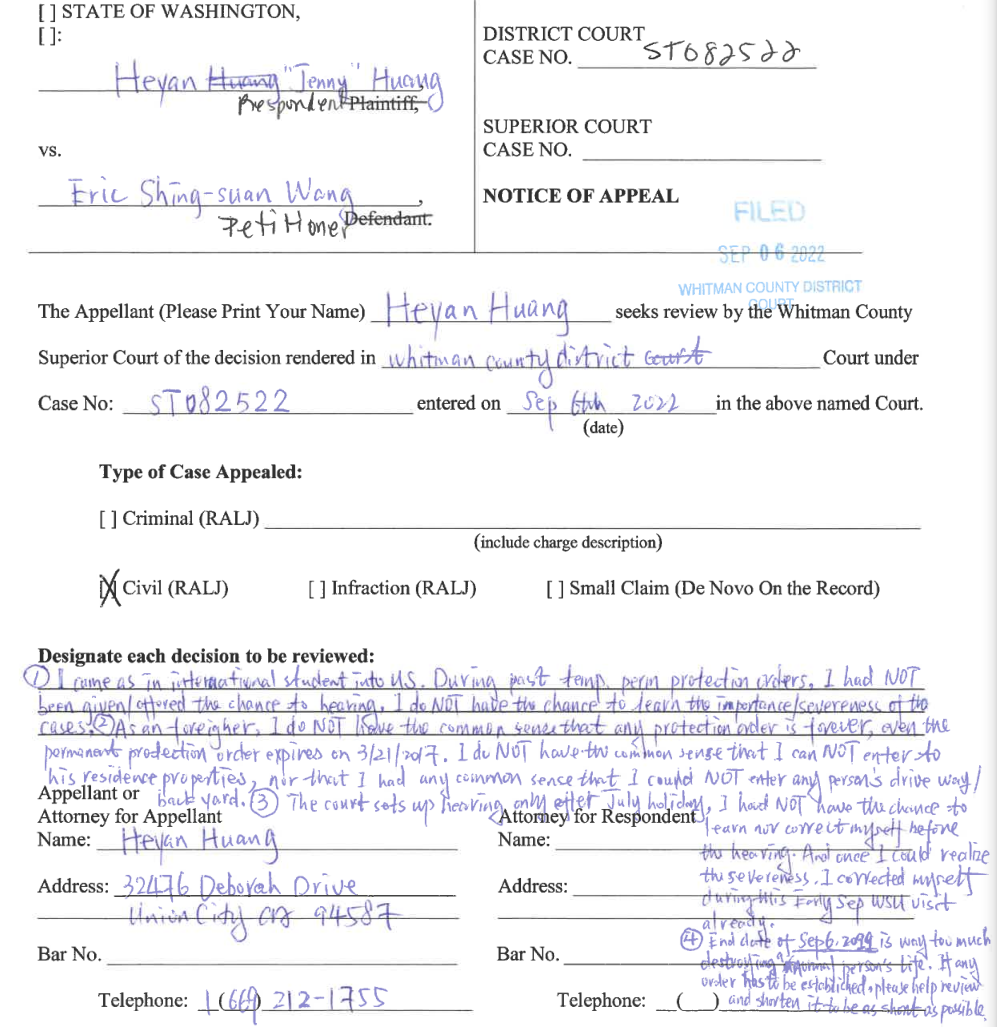
\includegraphics[width=.9\linewidth]{./pic/dearCousin_20220919_222530.png}
\begin{itemize}
\item You honor, I \textbf{filed my appeal the same day within 1st hour of effective Stalking protection order (Case No. ST082522) same day on Sep. 6, 2022}, as the \textbf{respnodent I am NOT able to accept the fact that another stalking protection order has been successfully setup against me when I am feeling it is mis-manipulated setting up, and needs to be reviewed}.
\item The judge has been in favor of petitioner's willings, but lack of consideration and all previous case handling towards response, which is unreasonable and unfair for respnodent.
\item There were tramandous mis-comunications and information interpreting upon most recent as well as previous mis-manipulated cases (\textbf{including but NOT limied to Case No. AH-0117YB}), that needs to be reviewed and reconsidered.
\item \textbf{Same day appealing filed TYPED REASONS LISTING}: Please forgive my same day filling of the appeal and the limited space urgly handwriting. I will copy and type all listed 4 reasons above here as followed:
\end{itemize}

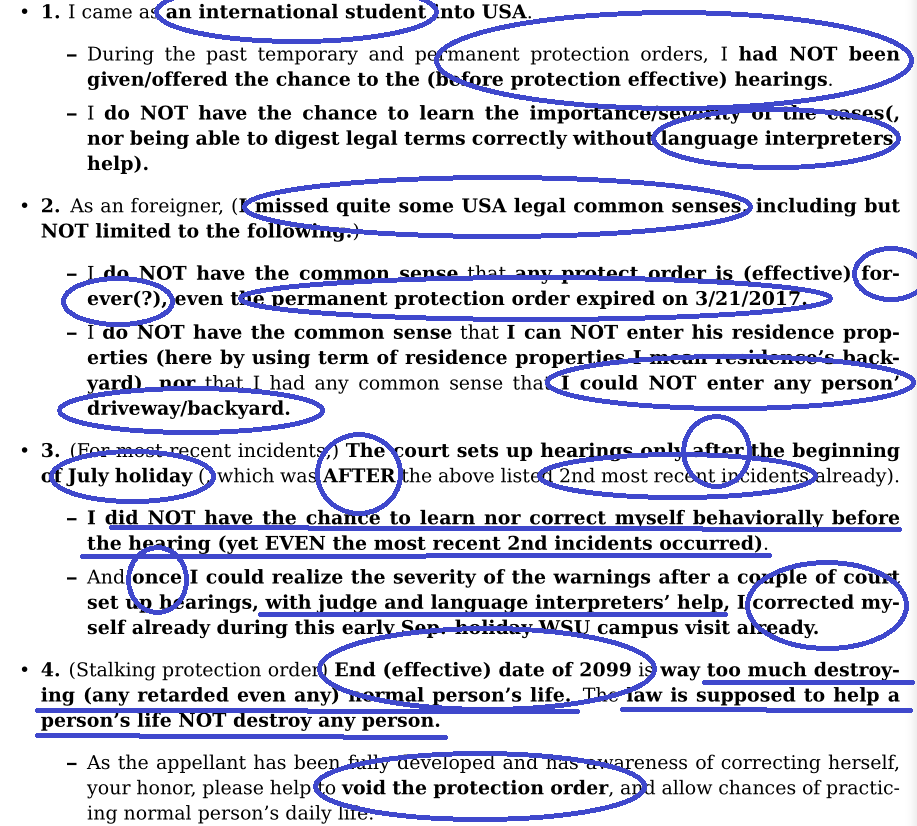
\includegraphics[width=.9\linewidth]{./pic/dearCousin_20220920_093957.png}

\section{Other court cases}
\label{sec-2}

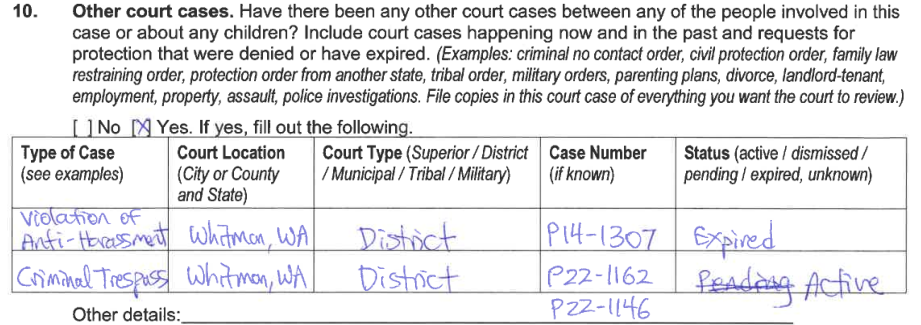
\includegraphics[width=.9\linewidth]{./pic/dearCousin_20220919_153339.png}
\subsection{There are 2 ACTIVE cases going on: \textbf{P22-1146} and \textbf{P22-1162};}
\label{sec-2-1}
\subsubsection{\textbf{P22-1146}}
\label{sec-2-1-1}

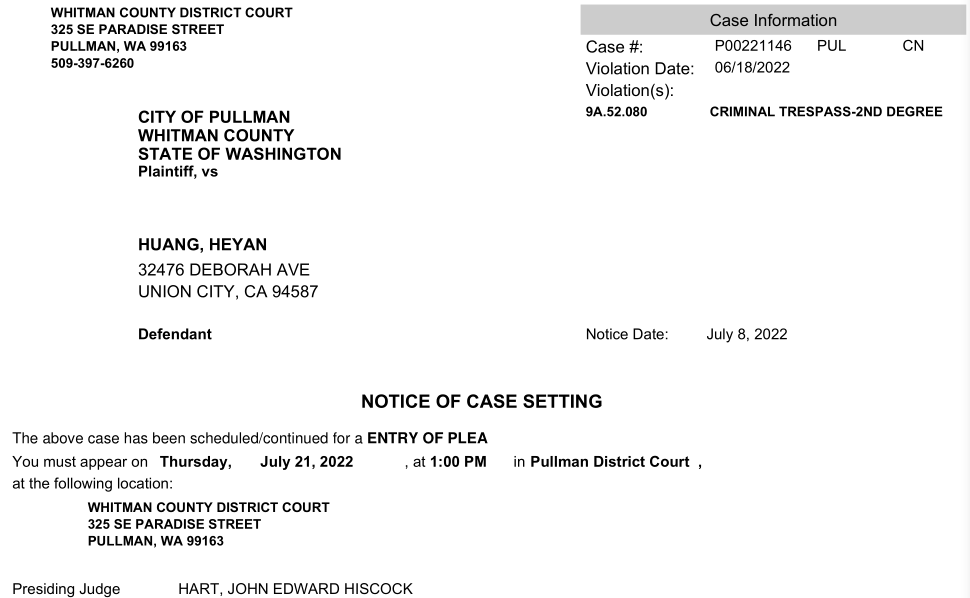
\includegraphics[width=.9\linewidth]{./pic/dearCousin_20220919_185022.png}
\begin{itemize}
\item Due to the slightly relatively late response of court arrangement of hearing, a person without necessary boundary understandings does NOT have the necessary chance in time to learn and self-correct his/her behavior after ONE such mistake.
\end{itemize}
\subsubsection{\textbf{P22-1162}}
\label{sec-2-1-2}

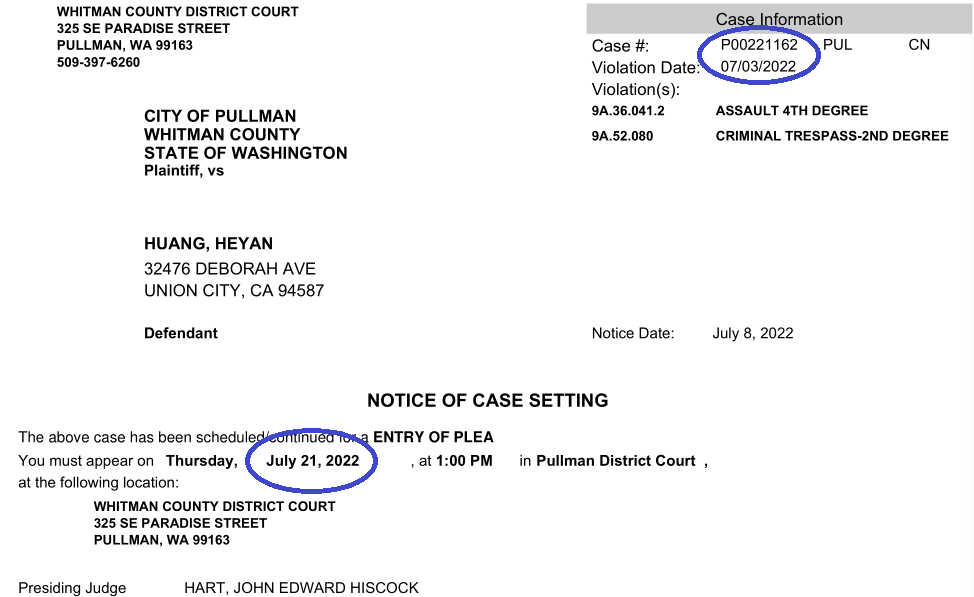
\includegraphics[width=.9\linewidth]{./pic/dearCousin_20220919_185057.png}
\begin{itemize}
\item There are 2 Active cases, but the cases were only taken care of \textbf{AFTER the second P22-1162 incident on 07/03/2022}, \textbf{which date for both cases were set up hearing on July 21, 2022, and noticed on July 8, 2022}, and which were after the 2nd incident and I would have NO chance/opportunity to learn nor correct myself without IN TIME hearing after 1st incident.
\end{itemize}
\subsubsection{There is 1 EXPIRED case of \textbf{P14-1307}}
\label{sec-2-1-3}
\begin{itemize}
\item As far as the protection order is expired, I \textbf{did have been interpreting expired protection orders as permission of retrying.}
\item \textbf{I need the court and judge to help me explain and understand what does expired protection orders mean to respnodent in NOT far future.}
\end{itemize}

\section{Length of Order}
\label{sec-3}

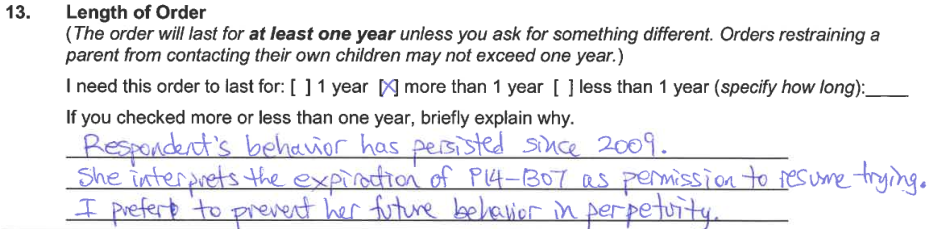
\includegraphics[width=.9\linewidth]{./pic/dearCousin_20220919_153711.png}
\begin{itemize}
\item Who came to US as an international student, \textbf{I do NOT have nor by any means learn and understand these legal terms}, and I \textbf{DO have BEEN INTERPRETING the EXPIREATION of P14-1307 as PERMISSION TO RESUME TRYING}. 
\begin{itemize}
\item \textbf{As an previous girl-friend who is still deeply falling in love for a previous boyfriend, who will stop trying by any means though?}
\item \textbf{Even the respondant I have been wrongly interpreting the legal terms and concepts}, what I need is \textbf{only someone, either the judge or the language interpreter to help correct me, instead of any life long life threatening permanent protection order.}
\end{itemize}
\item We understand petitioner's understandable intention, but \textbf{we also need to consider and allow the respnodent chance and opprotunities to grow, to learn as well as correct herself}, instead of setting up permanent protection orders without reasonable consideration on response's side of story and feelings.
\end{itemize}

\section{Most Recent Incidentn}
\label{sec-4}

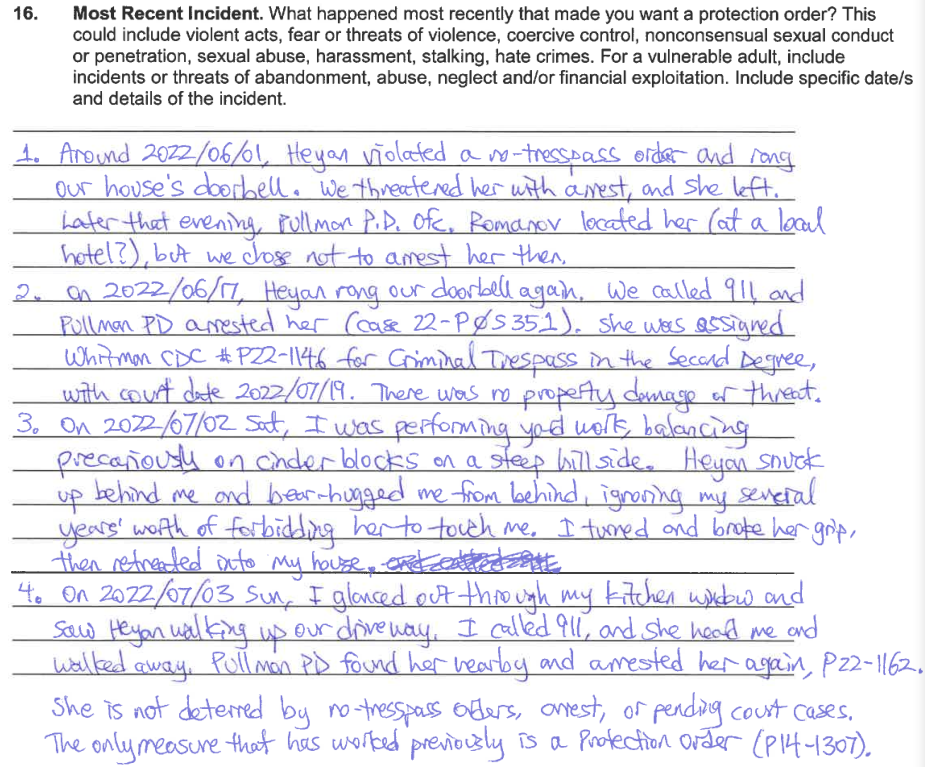
\includegraphics[width=.9\linewidth]{./pic/dearCousin_20220919_183412.png}
\begin{itemize}
\item Your honor, my explaination are as following listed:
\item 1. I \textbf{did have interpreted expired protection orders as permission of allowance for retrying during all past years without basic legal knowledge and common sense}. And it had been the reason that I had been visited back during 2021 upon which year I devorced ex-husband, and want to retry the relationship with Mr. Eric Shing-suan Wang. And I did have visted quite a few times back then, \emph{\textbf{2 times last year in 2021}}, in \textbf{end of March 2021}, \textbf{July 30th, 2021}, and followed with /*3 times visitings this years in \textbf{end of May}, \textbf{middle of June}, as well as \textbf{beginning of July.}
\item 1. I entered the place, but \textbf{there had been NO any valide no-trespass order against me. And the expired protection order was interpreted as permission of retrying in my mind and head.}
\item 1. \emph{\textbf{There was a policement did call me when I was about to register for a hotel room in end of May 2022}}, but \textbf{the unreasonable expiring date of 2099 the policeman warned me over the phone} made me believe that \textbf{it was more a threatens from a unprofessional small town policeman, which cases had happened on me before, on 12/27/2014 I had been arrested by unprofessional small town policeman who had absolutely no right to arrest me at that time, but he did.}
\item 2. I \textbf{was arrested by the policeman on 6/17/2022}. But your honor, please help consider the following stated facts:
\begin{itemize}
\item I \textbf{was raised up in a large family with 3 elder siblings, from a farm out of an undeveloped coutry}, whose parent did NOT know how to take good care of their children nor to look into their children's psychological growth;
\item \textbf{I had NOT been taken good care of during my childhood}, and \textbf{had been raised up with to some extend disability of missing concepts of various boundaries}.
\item I knew that \textbf{Mr. Eric Shing-suan Wang had verbally warned me NOT go to the house}, but back then \textbf{I was NOT able to understand how serious the warn could be and can NOT synchronize my behavior with the warned statements yet}.
\item And even at my age in my early forties, I am still practicing various boundaries during my daily life. \textbf{Personally I have been in great need of the court's hearings' help, judge's help to help behaviorly correct me and help me set up boundaries as well as help me understand how important and how severe things could potentially be.}
\end{itemize}
\item 3. Your honor, it was one of the afternoon that I have driven more than 1000 miles one way within less than 24 hours, and I was tired, only saw a person in between the two neighbourhood houses. As an international student, I don't have any concepts that I am NOT allowed to enter any household's backyard, not only Mr. Eric Shing-suan Wang's, and \textbf{it was in between open yards of two neighbourhood houses without any marks/WARNING stating NO ENTERING}, i was just trying to get close to see backyeard scene, but \textbf{due to the steep hillside and my tiredness, I run out of balance, and to prevent myself from falling and hitting onto hard steep hillside stones, I ended of snuck a person nearby, which turned out to be Mr. Eric Shing-suan Wang} whom I was warned NOT to touch on, but it was completely a situation of a very tired person running into out of balance emergency situations. Your honor, please help understand the tiredness of driving more than 1000 miles continuously within less than 24 hours. Thanks for your understanding so much!
\item 4. Your honor, \textbf{I was NOT intended to, and I had even driven more than 20 miles on my way back to CA, and I had even grabbed groceries (water) from neighbouring town} (Please check below receipt \textbf{form neighbouring town Colfax, WA} before the backed to Pullman arrestment). But due to the heavy rain which I had waited the whole day before I left for home that day, \textbf{experiencing the heavy rain on my way to Colfax, I decided to drive back to visit WSU campus after the raining when the campus was wet}. 
\begin{itemize}
\item As \textbf{an international foreigner who lacks some necessary common sense} and \textbf{do NOT know we are NOT supporse to walk onto any house's drive way}, I did walked onto \textbf{the drive way in between the 2 neighbouring house without thinking nor understanding the warnings fully} once more before I left for CA when the ground was wet, and walked my way away after having walked it once more when ground was wet.
\item And your honor, due the previously stated facts of \textbf{NOT BEING TAKEN GOOD CARE OF during my childhood} during which ages \textbf{I cried too much for years and had been seeing doctors for years for my ears}, I had significant obsererable ear problems for years when I was young, and later on when I grow up \textbf{I did notice that I have slightly hearing problems} (which was tested, 1st time noticed to me in classroom in one of my Computer Science majored course \textbf{in Fall 2013 or Fall 2014 semester}, that \textbf{I am NOT able to hear low volumes}; and at age of 43 I had obsererable significant eye floaters inside my current eyes since Aug. 2022, which can be side proof of my grown up environment as well), and \textbf{I actually did NOT hear nor notice any calling of 911 for policeman nor anything inside the house}.
\end{itemize}
\item I NEVER mean to do anything threatening nor damage anything to Mr. Eric Shing-suan Wang personally nor to the house properties around it.
\end{itemize}

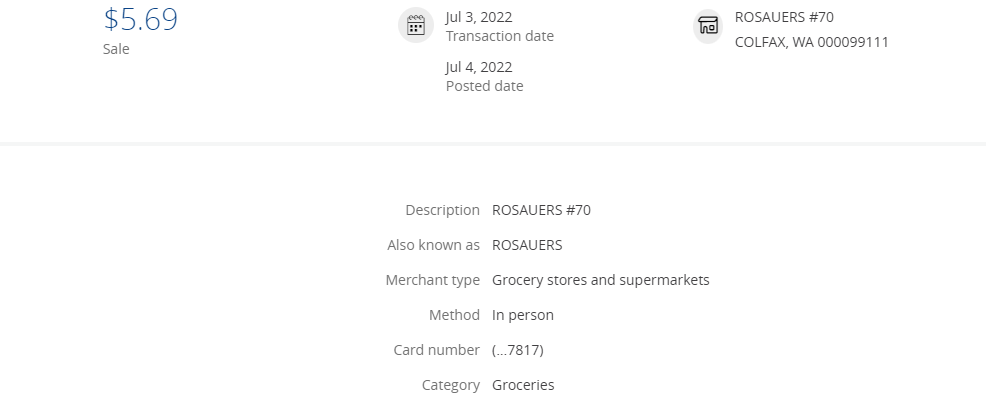
\includegraphics[width=.9\linewidth]{./pic/dearCousin_20220919_201117.png}
\section{Past Incidents}
\label{sec-5}

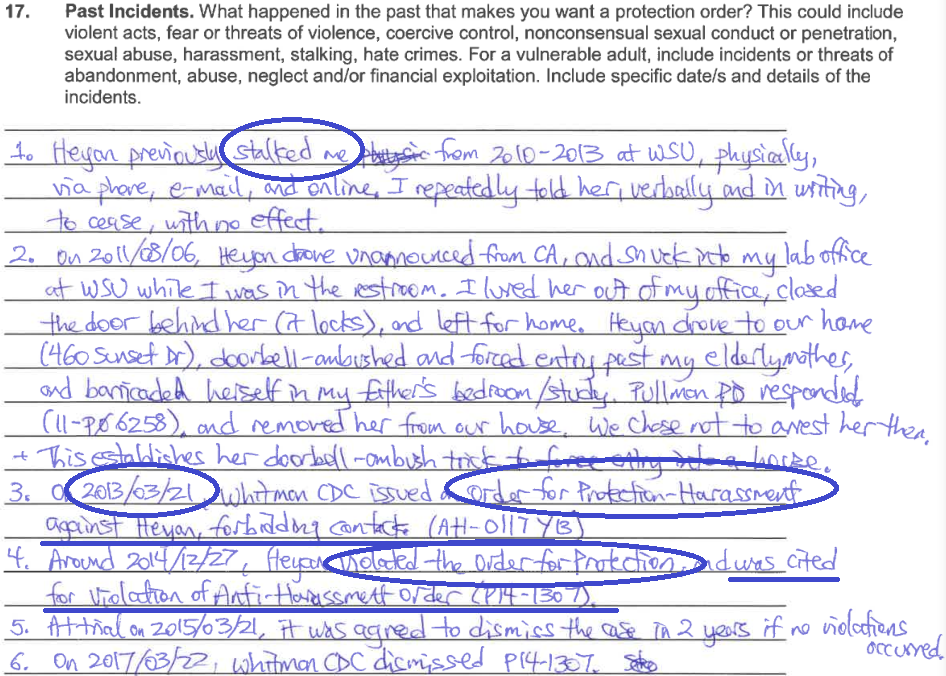
\includegraphics[width=.9\linewidth]{./pic/dearCousin_20220919_183625.png}
\begin{itemize}
\item Your honor, my explaination are as following listed:
\item 1. Your honor, back between 2010-2013, I was only in my early thirties. For other general majority of population, it must be an age of mature enough to handle things correctly and professionally, but for me personally as an slightly retarded, I was still naive, and with the missing boundaries concepts and understandings, I was sincerely NOT able to understand and digest what had been going on during those ages.
\item 2. Your honor, what was stated was completely correct, but \textbf{at that age I was NOT able to understand what's going on, nor be able to reasonably understand the relationships between boyfirend and girlfriend}. And the only fact I know is that \textbf{I love this person Mr. Eric Shing-suan Wang deep inside my heart, and without him being my future husband, the rest of my life will be someone else's, NOT mine, and I won't be happy for the rest of my WHOLE life.}
\item 3. \textbf{Case No. AH-0117YB ORDER FOR PROTECTION HARASSMENT was a completely mis-manipulated case executed upon me -- a naive international student}. 
\begin{itemize}
\item I have \textbf{NOT been notified any hearing for this Harassment protection order against me, nor had been served the protection order when it was effiective.}
\item I \textbf{was only able to get a copy on 12/29/2014 upon which day I had been arrested for this order}, and upon when I have NO idea about any protection order against me, only that the police who arrested me mentioned once that I could ask for the file when I were able to be bonded out of the jail on 12/29/2014.
\item \textbf{The protection order was finally served to me on court date 2/27/2015.} But \textbf{on 12/27/2014 the unreasonable arrestment had put me into all kinds of psychological problems the whole spring 2015 during my naive age when I was NOT able to digest the whole case and all the threatening it brought into my life.}
\item And \textbf{the protection order against me during my naive age eventually resulted in a mistaken unthoughtful marriage which I regret all the time and would wish I had never got maried once when I was NOT being able to digest the whole 4 years length protection order against me.}
\end{itemize}
\item 4. \textbf{I did visit Mr. Eric Shing-suan Wang's office on 12/27/2014. And got arrested that day same day}. But your honor, please help learn the facts stated above also that: 
\begin{itemize}
\item \textbf{I had NEVER been notified any protection order hearing, nor had been served any protection order file, and I had NO concepts NO impression about any protection order before 12/27/2014.}
\item My last case back then of \textbf{PC011713 was settled down on 3/7/2013, and the case would dismiss on 3/7/2014.}
\item At \textbf{an naive international student who was NOT able to digest the legal terms well nor had been able to get enough help either from the judge nor had been offered any language interpreters' help}, and I \textbf{did interpret it as after 3/7/2014, I would be permitted to retry. And I waited half more year (0.75 more year after 3/7/2014) till 12/27/2014 to retry and revisit Mr. Eric Shing-suan Wang's student office.} And I got arresteded.
\end{itemize}
\item 5. \textbf{I was formally served the protection order AH-0117YB} ORDER FOR PROTECTION HARASSMENT \textbf{on 2/27/2015}, and learned through a hard way that I was legally NOT permitted to visit Mr. Eric Shing-suan Wang at least before 3/21/2017. \textbf{And I may regain my permissions and retry afterwards (after 3/21/2017) if I want.}
\end{itemize}

\section{Stalking protection order No. ST082522}
\label{sec-6}

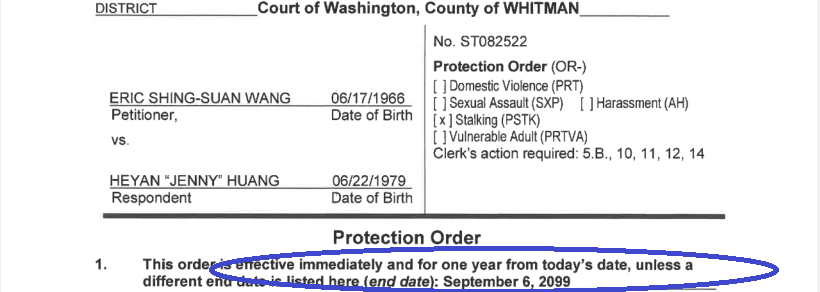
\includegraphics[width=.9\linewidth]{./pic/dearCousin_20220919_222725.png}
\begin{itemize}
\item With about 8-10 more years mature, this slow grown up naive female is finally able to digest necessary concepts with the court and judge as well as launguage interpreter's help. \textbf{And with a few court hearing dates setup and language interpreter's help since end of July the first hearing, I were able to understand and setup the necessary boundaries, and I learned what I could NOT behave towards Mr. Eric Shing-suan Wang when I have been warned NOT to do}.
\item \textbf{I have visited WSU campus during Sep 5 this year long week end}, and had stayed in town for more than 3 days in hotel. \textbf{I practiced and succeeded that I have NOT done anything wrong behaviorly toward this magical person Mr. Eric Shing-suan Wang during the visit, till the end of his protection order hearing and safely smoothly left the town for CA.}  

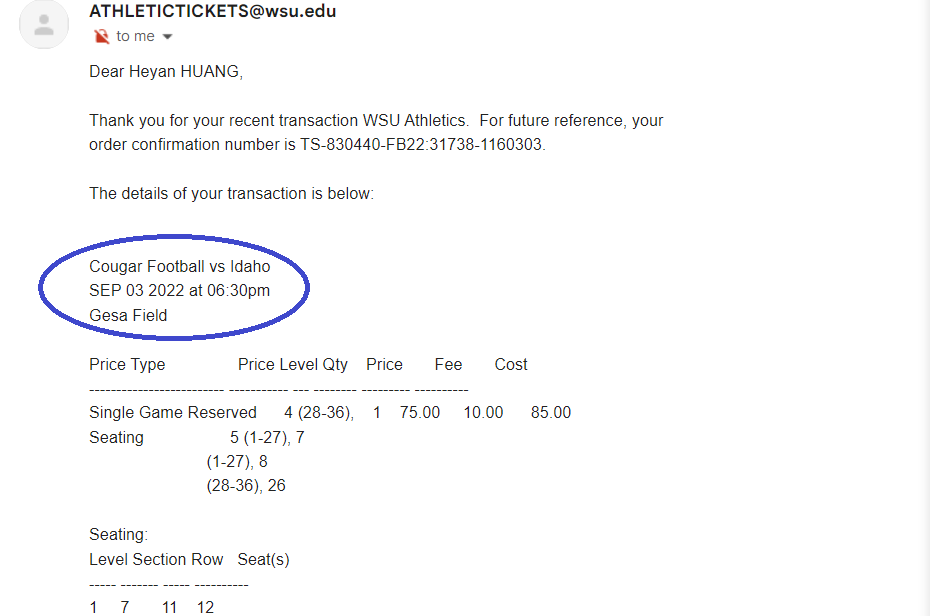
\includegraphics[width=.9\linewidth]{./pic/dearCousin_20220920_103727.png}
\item I did have stated the aboved mentioned \textbf{circumstances of my childhood growing up environment}, \textbf{personality missing boundaries concepts shortcomings}, \textbf{naiveness as well as mature grown up after 8-10 more years}, as well as \textbf{my behavior self-correcting after court hearings judge and launguage interpreters' help}, and \textbf{my most recent perfectly behaved visit and staying in town for quite a few days} during the protection order hearing date on Sep 6, 2022 on my turn, \textbf{the judge argued and emphasized that he listened and took notes on all of them}, but I do feel \textbf{the judge still does NOT consider my side of reasonings, and I have to state all of them clearly during the Appellant's desination here now.}
\item There is a famous WSU home game this weekend on 9/24/2022, which game I booked ticket for, and I will practice one more and a few more times (later this football game season in Oct. as well as Nov. 2022) to make sure that I learn and grow from this matter. 

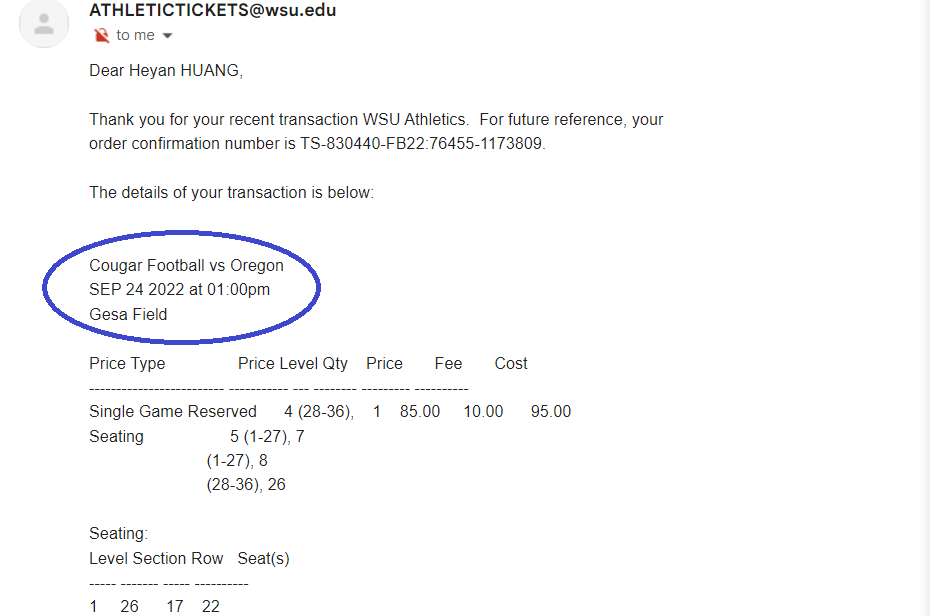
\includegraphics[width=.9\linewidth]{./pic/dearCousin_20220920_104317.png}
\item \textbf{I AM HAVING ABSOLUTE HARD TIME AND DIFFICUTLY UNDERSTANDING why any protection order would last till 2099 when right now it is only 2022, and there are 77 years to go for a stalking order} when \textbf{respnodent is a to some extent RETARDED} with \textbf{recent years' full development and mature, and powered up with self-awareness and self behavior correcting.}
\end{itemize}
% Emacs 27.1 (Org mode 8.2.7c)
\end{document}